%% LyX 2.2.1 created this file.  For more info, see http://www.lyx.org/.
%% Do not edit unless you really know what you are doing.
\documentclass[12pt]{article}
\usepackage[latin9]{inputenc}
\usepackage{geometry}
\geometry{verbose,tmargin=25mm,bmargin=0cm,lmargin=28mm,rmargin=0cm}

\makeatletter

%%%%%%%%%%%%%%%%%%%%%%%%%%%%%% LyX specific LaTeX commands.
%% Because html converters don't know tabularnewline
\providecommand{\tabularnewline}{\\}

%%%%%%%%%%%%%%%%%%%%%%%%%%%%%% User specified LaTeX commands.
\usepackage{tikz}
\usetikzlibrary{calc}
\usetikzlibrary{shapes}
\usepackage{mathrsfs}
\usepackage{mathabx}
\usepackage{txfonts}
\usepackage{pxfonts}
\usepackage{titling}
\usepackage{array}

\newdimen\un
\un=.8mm
\def\bordure{
\begin{tikzpicture}[overlay,remember picture]
\def\p{.75}
\def\ang{45}
\def\alp{160.2}
\def\bet{72.42}
\def\gam{-13.2}
\draw [very thick, line width = 8pt, color = red!25!blue!33.333!green!50]
($(current page.north west)+(20*\un,-20*\un)$)
-- ($(current page.north east)+(-24*\un,-20*\un)$)
node [draw, ellipse, fill, text=white, pos=.5] {\thetitle}
arc (90 : 0 : 4*\un)
-- ($(current page.south east)+(-20*\un,24*\un)$)
node[text=white,pos=.63 , rotate=90]
{\tiny Ce document est sous licence GNU FDL,
 il est librement modifiable et distribuable.
 Sources et licence compl�tes disponible sur le site.
 Copyright 2010, Jean-Christophe Jameux}
arc (0 : -90 : 4*\un)
-- ($(current page.south west)+(24*\un,20*\un)$)
node[draw, ellipse, fill, text=white, pos=.29] {\Large\bf Echologie.org}
arc (-90 : -180 : 4*\un)
-- ($(current page.north west)+(20*\un,-20*\un)$);

\un=1.3mm
\node(Triskell) at ($(current page.north west)+(16*\un,-12*\un)$){};
\draw [fill = white, color = red!25!blue!33.333!green!50]
(Triskell) + (1.2*\un,-6*\un) circle (15*\un);
\draw [fill = white, color = white] (Triskell) circle (2*\un);
\draw [fill = white, color = white]
(Triskell) + ({120*(1+\p)} : 3*\un)
arc ({120*(1+\p)} : 120 : 3*\un)
arc (180+\ang : 180-\ang :3*\un)
arc (\alp-\ang : \alp+\ang+24.8 : 5*\un);
\draw [fill = white, color = white]
(Triskell) + (120*\p : 3*\un)
arc (120*\p : 0 : 3*\un)
arc (90+\ang : 90-\ang : 6*\un)
arc (\bet-\ang : \bet+\ang+5.9 : 8*\un);
\draw [fill = white, color = white]
(Triskell) + ({120*(2+\p)} : 3*\un)
arc ({120*(2+\p)} : 240 : 3*\un)
arc (\ang : -\ang : 12*\un)
arc (\gam-\ang : \gam+\ang+.85 : 13*\un);
\end{tikzpicture}}

\makeatother

\begin{document}
\title{\LARGE\bf D�riv�es usuelles}

\parindent0cm \setlength{\extrarowheight}{12mm} \tabcolsep7mm 

{\LARGE{}}%
\begin{tabular}{ccc|cr}
 & {\LARGE{}$f\left(x\right)$} & {\LARGE{}$f'\left(x\right)$} & {\LARGE{}$f\left(u\right)$ } & {\LARGE{}
\begin{tikzpicture} [{shift=(1.5,.6)}, overlay]
	\draw [ball color = green, rotate = -16, scale = .6, opacity = .2 ] (0,0)
		 .. controls +(0,2)
 and +(0,2)  .. (3,0) 		 .. controls +(0,-2) and +(0,2)  .. (0,-4) 		 .. controls +(0,2)  and +(0,-2) .. (-3,0) 		 .. controls +(0,2)  and +(0,2)  .. (0,0);
 \end{tikzpicture} \begin{tikzpicture}[{shift=(-.5,-2.3)}, overlay]
	    \node(kinder){\hsize13cm\vbox{
			\begin{center}
			    \small
				$u$ est une variable d�pendant de $x$
				\par(i.e. une parenth�se contenant $x$)
				\par $u'$ d�signe la d�riv�e de $u$
				par rapport � $x$
			\end{center}		                		}};
\end{tikzpicture} $f'\left(u\right)\cdot u'$}\tabularnewline
{\LARGE{}\begin{tikzpicture}[scale=.5,overlay]
		\draw[->,>=latex](-1,0) --(1,0);
		\draw[->,>=latex](0,-1) -- (0,1);
		\draw(-1.1,0.4)--(1.1,0.4);
\end{tikzpicture}	} & {\LARGE{}$k$ } & {\LARGE{}0 } &  & \tabularnewline
{\LARGE{}\begin{tikzpicture}[scale=.5,overlay]
		\draw[->,>=latex](-1,0) --(1,0);
		\draw[->,>=latex](0,-1) -- (0,1);
		\draw(-1,-1)--(1,1);
\end{tikzpicture}	} & {\LARGE{}$x$ } & {\LARGE{}1 } &  & \tabularnewline
{\LARGE{}\begin{tikzpicture}[scale=.25,overlay]
		\draw[->,>=latex](-2,0) -- (2,0);
		\draw[->,>=latex](0,-2) -- (0,2);
		\draw plot[domain=-1.7:1.7](\x,\x*\x);
\end{tikzpicture}	} & {\LARGE{}$x^{2}$ } & {\LARGE{}$2x$ } & {\LARGE{}$u^{2}$ } & {\LARGE{}$2u\cdot u'$ }\tabularnewline
{\LARGE{}\begin{tikzpicture}[scale=.25,overlay]
		\draw[->,>=latex](-2,0) --(2,0);
		\draw[->,>=latex] (0,-2) -- (0,2);
		\draw plot[domain=-1.3:1.5](\x,\x^3);
\end{tikzpicture}	} & {\LARGE{}$x^{3}$ } & {\LARGE{}$3x^{2}$ } & {\LARGE{}$u^{3}$ } & {\LARGE{}$3u^{2}\cdot u'$ }\tabularnewline
{\LARGE{}\begin{tikzpicture}[scale=.25,overlay]
		\draw[->,>=latex](-2,0) --(2,0);
		\draw[->,>=latex] (0,-2) -- (0,2);
		\draw plot[domain=0:1.3](\x,\x^4);
		\draw[dashed] plot[domain=-1.25:0](\x,\x^4);
		\draw[dashed] plot[domain=-1.25:0](\x,{0-(\x^4)});
\end{tikzpicture}	} & {\LARGE{}$x^{n}$ } & {\LARGE{}$nx^{n-1}$ } & {\LARGE{}$u^{n}$ } & {\LARGE{}$nu^{n-1}\cdot u'$ }\tabularnewline
{\LARGE{}\begin{tikzpicture}[scale=.1,overlay]
		\draw[->,>=latex](-5,0) --(5,0);
		\draw[->,>=latex](0,-5) -- (0,5);
		\draw plot[domain=-5:-.2](\x,1/\x);
		\draw plot[domain=0.2:5](\x,1/\x);
\end{tikzpicture}	} & {\LARGE{}${\displaystyle \frac{1}{x}}$ } & {\LARGE{}$-{\displaystyle \frac{1}{x^{2}}}$ } & {\LARGE{}${\displaystyle \frac{1}{u}}$ } & {\LARGE{}$-{\displaystyle \frac{1}{u^{2}}\cdot u'}$ }\tabularnewline
{\LARGE{}\begin{tikzpicture}[scale=.25,overlay]
		\draw[->,>=latex](-2,0) -- (2,0);
		\draw[->,>=latex](0,-2) -- (0,2);
		\draw plot[domain=0:1.7](\x^2,\x);
\end{tikzpicture}	} & {\LARGE{}$\sqrt{x}$ } & {\LARGE{}${\displaystyle \frac{1}{2\sqrt{x}}}$ } & {\LARGE{}$\sqrt{u}$ } & {\LARGE{}${\displaystyle \frac{1}{2\sqrt{u}}\cdot u'}$ }\tabularnewline
{\LARGE{}\begin{tikzpicture}[scale=.1,overlay]
		\draw plot[smooth,domain=-3:1.8] (1.5*\x,2.718281828^\x);
		\draw[->,>=latex] (-5,0) -- (5,0);
		\draw[->,>=latex] (0,-5) -- (0,5);
\end{tikzpicture}	} & {\LARGE{}$e^{x}$ } & {\LARGE{}$e^{x}$ } & {\LARGE{}$e^{u}$ } & {\LARGE{}$e^{u}\cdot u'$ }\tabularnewline
{\LARGE{}\vphantom{{\LARGE{}$\frac{1}{\frac{1}{\frac{1}{1}}}$}}\begin{tikzpicture}[scale=.1,overlay]
		\draw plot[smooth,domain=-3:1.8] (2.718281828^\x,1.5*\x);
		\draw[->,>=latex] (-5,0) -- (5,0);
		\draw[->,>=latex] (0,-5) -- (0,5);
\end{tikzpicture}	} & {\LARGE{}$\ln x$ } & {\LARGE{}${\displaystyle \frac{1}{x}}$ } & {\LARGE{}$\ln u$ } & {\LARGE{}${\displaystyle \frac{1}{u}\cdot u'}$ }\tabularnewline
\hline 
 & {\LARGE{}$ku$ } & {\LARGE{}$ku'$ } & {\LARGE{}$uv$ } & {\LARGE{}$u'v+uv'$ }\tabularnewline
 & {\LARGE{}$u+v$ } & {\LARGE{}$u'+v'$ } & {\LARGE{}${\displaystyle \frac{u}{v}}$ } & {\LARGE{}${\displaystyle \frac{u'v-uv'}{v^{2}}}$}\tabularnewline
\end{tabular}{\LARGE \par}

\bordure
\end{document}
